%% LyX 2.3.6 created this file.  For more info, see http://www.lyx.org/.
%% Do not edit unless you really know what you are doing.
\documentclass[english,aspectratio=169]{beamer}
\usepackage{lmodern}
\renewcommand{\sfdefault}{lmss}
\renewcommand{\ttdefault}{lmtt}
\usepackage[T1]{fontenc}
\usepackage[latin9]{inputenc}
\setlength{\parskip}{\medskipamount}
\setlength{\parindent}{0pt}
\usepackage{amssymb}
\usepackage{graphicx}
\PassOptionsToPackage{normalem}{ulem}
\usepackage{ulem}

\makeatletter

%%%%%%%%%%%%%%%%%%%%%%%%%%%%%% LyX specific LaTeX commands.
\pdfpageheight\paperheight
\pdfpagewidth\paperwidth


%%%%%%%%%%%%%%%%%%%%%%%%%%%%%% Textclass specific LaTeX commands.
% this default might be overridden by plain title style
\newcommand\makebeamertitle{\frame{\maketitle}}%
% (ERT) argument for the TOC
\AtBeginDocument{%
  \let\origtableofcontents=\tableofcontents
  \def\tableofcontents{\@ifnextchar[{\origtableofcontents}{\gobbletableofcontents}}
  \def\gobbletableofcontents#1{\origtableofcontents}
}

%%%%%%%%%%%%%%%%%%%%%%%%%%%%%% User specified LaTeX commands.
\usetheme{CambridgeUS}
\usecolortheme{dolphin}
\hypersetup{pdfpagemode=None}
\usepackage{tikz}
\usepackage{color}
\usepackage{listings}

\makeatother

\usepackage{babel}
\begin{document}
\title[M3-2]{Eulerian and Lagrangian motion}
\author{Department of Oceanography}
\institute[UCT]{University of Cape Town}
\date{SEA3004F}
\makebeamertitle

\section*{Outlines}
\begin{frame}{Outline}

\tableofcontents{}
\end{frame}


\section{The continuum hypothesis and fluid parcels}
\begin{frame}{The continuum hypothesis}
\begin{columns}[t]

\column{5.5cm}

{\scriptsize{}One main assumption of fluid dynamics is that fluids
can be treated as continuum objects. Their properties, such as water
density, are assumed to have an interval of volume over which the
density estimate does not change with the size of the sampling. }{\scriptsize\par}

{\scriptsize{}At the microscopic range (}\textbf{\scriptsize{}region
A}{\scriptsize{}), the sampling of density is affected by the fluctuation
in the number of molecules observed. In }\textbf{\scriptsize{}region
C}{\scriptsize{}, the variation is due to the macroscopic spatial
distribution of density, like measuring different water masses. In
}\textbf{\scriptsize{}region B}{\scriptsize{}, at the scale of water
parcels, we measure the ``local mean value'' of density (from Batchelor). }{\scriptsize\par}

\column{10cm}

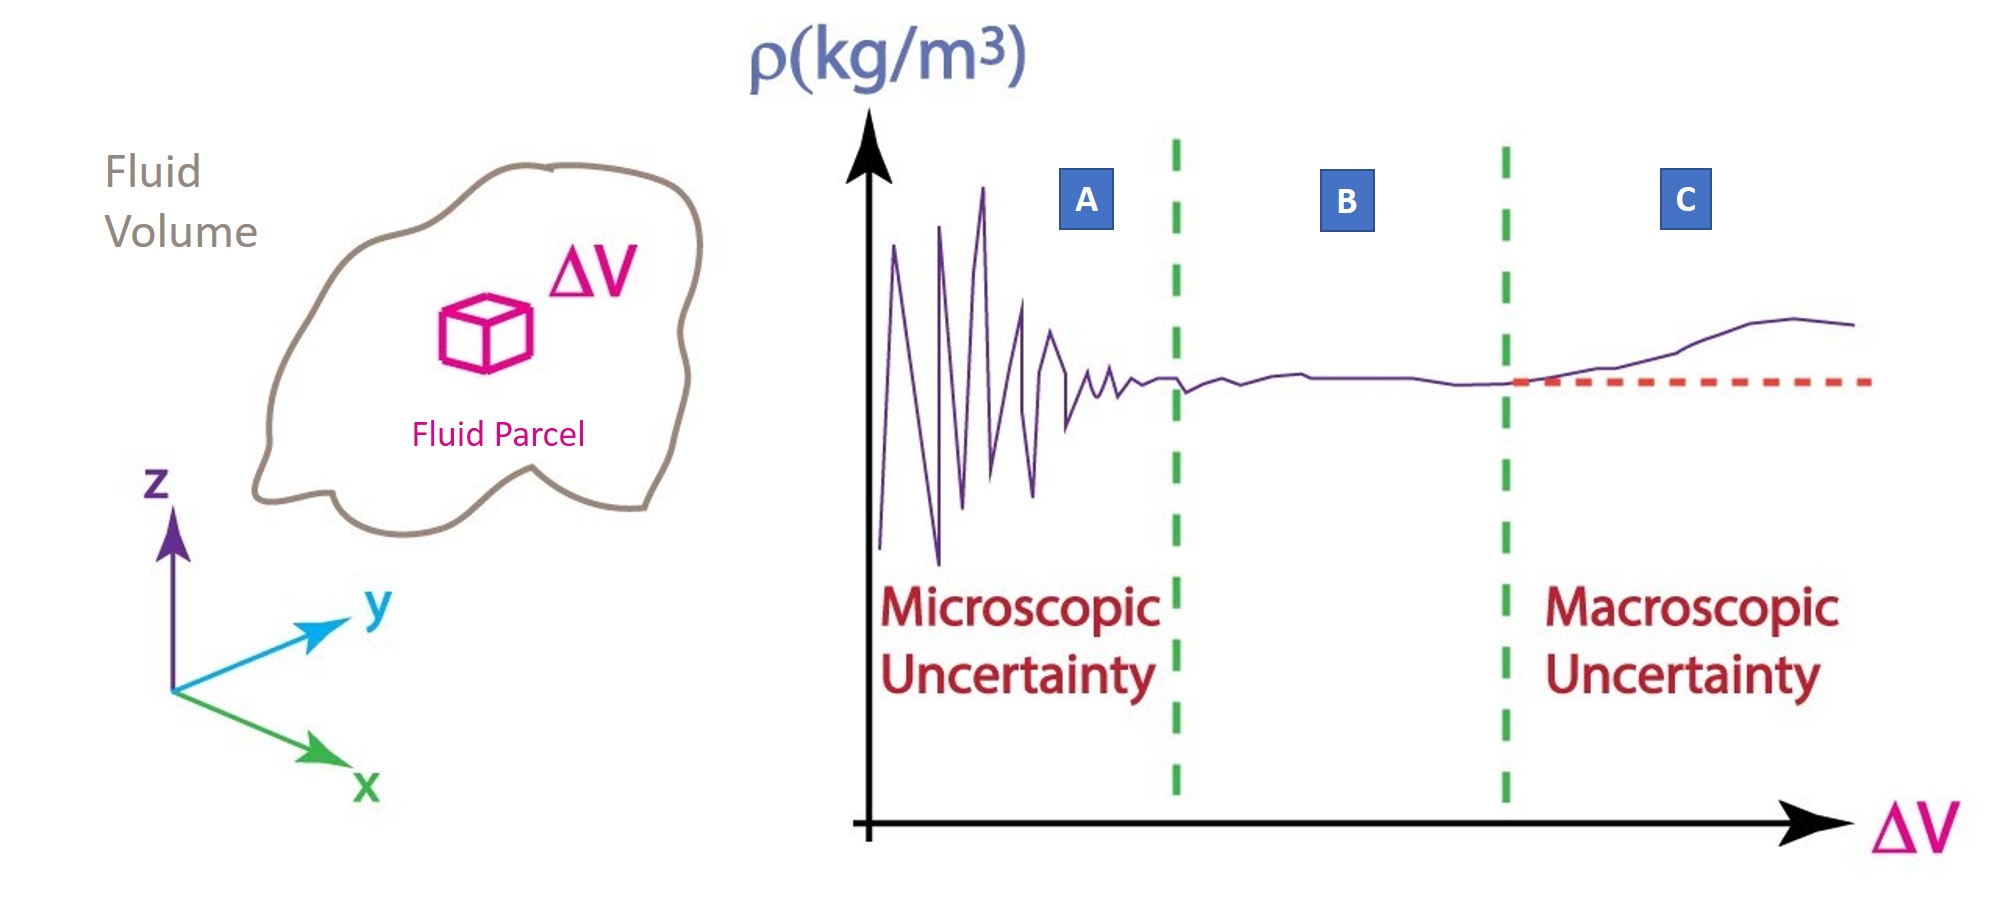
\includegraphics[width=10cm]{figures/M3/continuum_hypothesis}
\end{columns}

\end{frame}

\begin{frame}{The fluid parcel}

\begin{columns}[t]


\column{8cm}

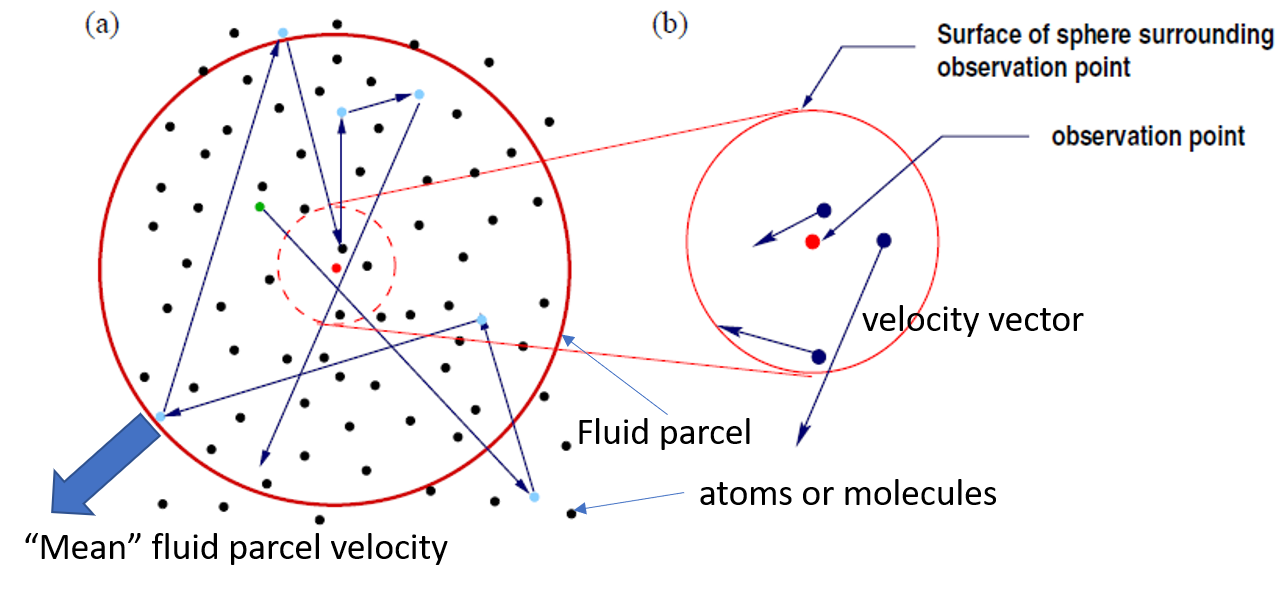
\includegraphics[width=7cm]{figures/M3/fluid_parcel}

{\scriptsize{}A fluid is composed of many molecules or atoms, each
one affected by random motion at the microscopic scale (fig. a). If
we compute the average velocity over a volume that is too small (fig.
b), we will capture only a few molecules and they will not be representative
of the mean velocity. We need to consider a volume that is }\textbf{\scriptsize{}sufficiently
big to capture the macroscopic features of the fluid}{\scriptsize{}.}{\scriptsize\par}

{\scriptsize{}The fluid parcel is a }\textbf{\scriptsize{}theoretical
construct}{\scriptsize{} that helps to understand and represent quantitatively
the fluid properties (figure from Lectures in Elementary Fluid Dynamics,
J. M. McDonough)}{\scriptsize\par}

\column{5cm}

{\scriptsize{}A fluid parcel can have any size and shape, but must
satisfy the following requirements, which constitute the continuum
hypothesis of fluids}{\scriptsize\par}
\begin{itemize}
\item {\scriptsize{}the volume of the fluid parcel is big enough to remove
the microscopic fluctuations but small enough to capture the larger
scale variations }{\scriptsize\par}
\item {\scriptsize{}its macroscopic properties (velocity, density, concentration
of a given substance) are representative of the bulk fluid at the
location of the parcel}{\scriptsize\par}
\item {\scriptsize{}there are infinite fluid parcels and the properties
of the fluid vary smoothly between one fluid parcel and the adjacent
ones}{\scriptsize\par}
\end{itemize}
\end{columns}

\end{frame}


\section{Lagrangian and Eulerian viewpoints }
\begin{frame}{Lagrangian and Eulerian representations}

A fluid can be described as a continuum object, in which we can deploy
instruments at every random position and obtain information. 
\begin{itemize}
\item \textbf{Eulerian representation}: equivalent to sampling the ocean
by using fixed moorings, or the atmosphere by using a fixed network
of weather stations. 
\item \textbf{Lagrangian representation}: to sample the ocean by following
the flow field, like using floats or balloons. 
\end{itemize}
\textbf{The fluid is however the same}, and the two ways of observing
it must return the same motion (though complementary information).
The historical video in the supporting material illustrates the problem
at large.
\end{frame}


\section{The Eulerian derivative}
\begin{frame}{The Eulerian derivative: measuring change at fixed points}

\begin{columns}[t]


\column{7.5cm}

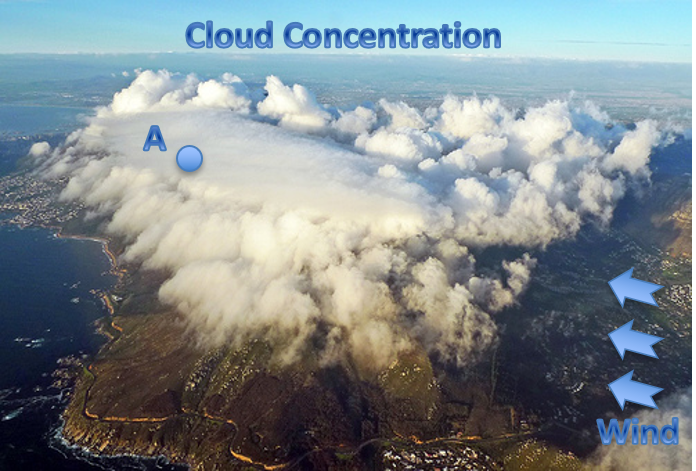
\includegraphics[width=7cm]{figures/M3/table-cloth_A}

{\scriptsize{}Cloud cover can be seen as a 4-D field $C=C\left(x,y,z,t\right)$
measured in \%. A fixed observer at site $A\equiv\left(x_{A},y_{A},z_{A}\right)$
on top of Table Mountain measures $C_{A}=C\left(x_{A},y_{A},z_{A},t\right)$.
This is a time series of cloud cover, due to the various fluid parcels
passing through the point }{\scriptsize\par}

\column{6cm}
\begin{itemize}
\item {\scriptsize{}The rate of change at any fixed point is called the
}\textbf{\scriptsize{}Eulerian derivative}{\scriptsize{}
\[
\left(\frac{\partial C}{\partial t}\right)_{point}
\]
You should note that the Eulerian derivative is also a scalar field,
and we are just looking at one of its infinite points.}{\scriptsize\par}
\item {\scriptsize{}In this example, we can assume that cloud concentration
is rather constant over a certain amount of time at point A. Observer
A will not see much change in cloudiness, so that 
\[
\left(\frac{\partial C}{\partial t}\right)_{point}=0
\]
}{\scriptsize\par}
\end{itemize}
\end{columns}

\end{frame}

\begin{frame}{The fluid parcel view point}

\begin{columns}[t]


\column{7.5cm}

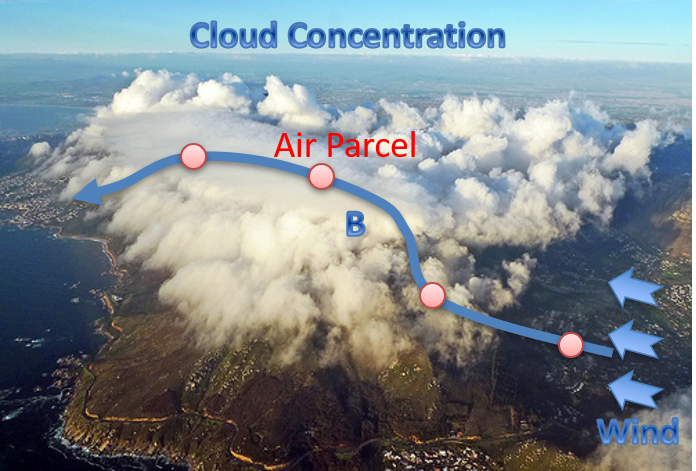
\includegraphics[width=7cm]{figures/M3/table-cloth_B}
\begin{itemize}
\item {\scriptsize{}We now look at individual parcels. All fluid parcels
are pushed by the wind and raised by the topography, so they follow
a path similar to the one shown in B}{\scriptsize\par}
\end{itemize}

\column{6cm}
\begin{itemize}
\item {\scriptsize{}As the parcel moves upwards into lower pressures, it
expands and cools adiabatically (see Module 2). }\textbf{\scriptsize{}Water
vapour condenses forming clouds and $C$ increases}{\scriptsize{}.
At the end of the mountain the parcel sinks down because its colder
than the surrounding. It warms, the }\textbf{\scriptsize{}water goes
back to the gaseous phase, the cloud disappears and $C$ decreases}{\scriptsize{}.}{\scriptsize\par}
\item {\scriptsize{}When we follow the parcel trajectory the rate of change
is thus not constant:}
\[
\left(\frac{\partial C}{\partial t}\right)_{parcel}\ne0
\]
\end{itemize}
\end{columns}

\end{frame}


\section{The Lagrangian view point}
\begin{frame}{The Lagrangian framework}

\begin{columns}[t]


\column{7.5cm}

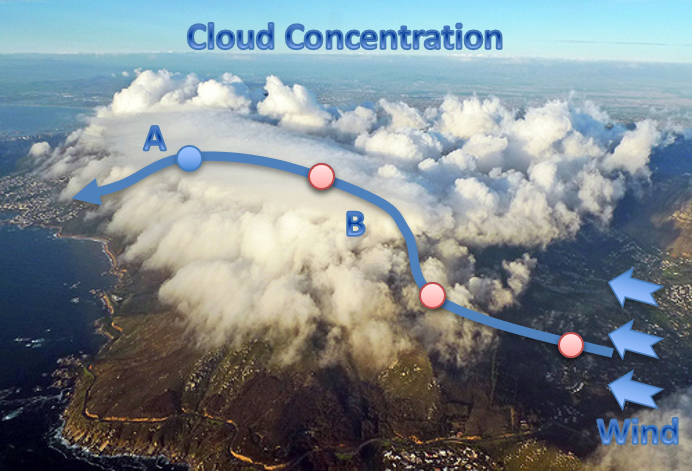
\includegraphics[width=8cm]{figures/M3/table-cloth_A&B}

\column{6cm}
\begin{itemize}
\item {\scriptsize{}When the trajectory B crosses point A, we must describe
the same phenomenon and have the same concentration over time. (The
cloud field is the same after all, it is just the way we observe it
that changes)}{\scriptsize\par}
\item {\scriptsize{}How can we reconcile the two different ways? How do
we express the rate of change taking into account the movement of
the fluid? }{\scriptsize\par}
\item {\scriptsize{}We need a special way to represent the changes, }\textbf{\scriptsize{}the
Lagrangian derivative}{\scriptsize\par}
\end{itemize}
\end{columns}

\end{frame}

\begin{frame}{The derivative following the fluid parcel}

\begin{itemize}
\item {\small{}Change in a function of multiple variables like $C=C\left(x,y,z,t\right)$
can be expressed as 
\begin{equation}
\delta C=\frac{\partial C}{\partial t}\delta t+\frac{\partial C}{\partial x}\delta x+\frac{\partial C}{\partial y}\delta y+\frac{\partial C}{\partial z}\delta z\label{eq:differential}
\end{equation}
where the partial derivatives indicate that we are only computing
the rate of change due to that independent variable $(x,y,z,t)$.}{\small\par}
\item {\small{}The parcel is moving according to a velocity vector field
$\mathbf{u}=\left(u,v,w\right)$. The spatial changes of the parcel
positions can be written as $\delta x=u\delta t$, $\delta y=v\delta t$
and $\delta z=w\delta t$}{\small\par}
\item {\small{}The derivative following the parcel is obtained by substituting
the terms above in eq. (\ref{eq:differential}) and obtaining a new,
more comprehensive form of the time derivative
\[
\delta C=\left(\frac{\partial C}{\partial t}+u\frac{\partial C}{\partial x}+v\frac{\partial C}{\partial y}+w\frac{\partial C}{\partial z}\right)\delta t
\]
\begin{equation}
\frac{DC}{Dt}=\frac{\partial C}{\partial t}+u\frac{\partial C}{\partial x}+v\frac{\partial C}{\partial y}+w\frac{\partial C}{\partial z}\label{eq:total_derivative}
\end{equation}
}{\small\par}
\end{itemize}
\end{frame}


\section{The total derivative}
\begin{frame}{The total derivative operator}

\begin{itemize}
\item The operator $D/Dt$ is called the \textbf{total derivative} (other
names are \emph{Lagrangian} or \emph{substantial} or \emph{material})
and expresses the change in the properties of a fluid parcel in terms
of the Eulerian fields (the scalar $C$ and the vector $\mathbf{u}$
in our case)
\item Using the nabla operator and the definition of scalar product, the
vector form of eq. (\ref{eq:total_derivative}) becomes
\begin{equation}
\frac{DC}{Dt}=\frac{\partial C}{\partial t}+\mathbf{u}\cdot\nabla C
\end{equation}
\item The total derivative operator $D/Dt$ is used to \textbf{express the
change of any fluid property over time} due to local and/or advective
(transport) processes. This can be its temperature, pressure, concentration
of chemical or biological substances, \uline{and the fluid velocity
itself}
\end{itemize}
\end{frame}


\end{document}
